% !TEX root = ../main.tex

\section{Benchmark and Evaluation Details}
\label{app:benchmarks}

Across all three benchmarks, tasks are evaluated in chronological order. The solver receives task $x_i$ with only the information available before its release time, while the evolver receives outcome labels only after the corresponding resolution time. The table generator loads the first record for each \texttt{instance\_id}, so retries or duplicate logs do not change the reported metrics. The three datasets are finite evaluated prefixes of unbounded task streams and jointly cover the three deployment challenges in \S\ref{sec:intro}: stream continuation (D1), within-stream heterogeneity (D2), and temporal shift (D3).

\subsection{PolyBench}

\noindent\textbf{Source and composition.}
PolyBench is a Polymarket-derived prediction-market stream with 5{,}075 binary-outcome tasks from Feb 6--22, 2026. The stream spans politics, sports, finance, crypto, and entertainment markets, and each task is resolved against the official market outcome.

\noindent\textbf{Temporal ordering.}
For each market, we store the task release timestamp and the outcome resolution timestamp. Retrieval evidence is filtered by release time during solving. Resolved labels are hidden from evolution until the corresponding market has resolved.

\noindent\textbf{Metrics.}
Let $\mathcal{T}$ be the set of executed trades, excluding gated tasks, empty decisions, and \textsc{Skip} decisions. Let $s_i$ indicate whether trade $i$ is correct, $b_i$ be its confidence-weighted investment, and $g_i$ be its realized profit. The metrics reported for PolyBench are:
\begin{align*}
\mathrm{Acc} &= 100 \cdot \tfrac{1}{N}\textstyle\sum_{i\in\mathcal{T}} s_i \\
\mathrm{CWR} &= 100 \cdot \tfrac{\sum_{i\in\mathcal{T}} g_i}{\sum_{i\in\mathcal{T}} b_i} \\
\mathrm{Return} &= \tfrac{|\mathcal{T}|}{N}\cdot\mathrm{CWR}.
\end{align*}
Accuracy therefore rewards both broad coverage and correct decisions, while Return scales the portfolio profit-to-investment ratio by the fraction of tasks actually traded.

\subsection{CTF-Dojo}

\noindent\textbf{Source and composition.}
CTF-Dojo is a 261-challenge security-competition stream drawn from \texttt{pwncollege/ctf-archive}, chronologically ordered from 2011 to 2024. Challenges cover binary exploitation, web security, cryptography, reverse engineering, and forensics, exposing changes in challenge style and tooling over time.

\noindent\textbf{Sandbox and verification.}
Each challenge runs inside a per-task Docker sandbox with constrained network policy. Flags are submitted as text and verified by SHA-256 hash comparison against the official flag.

\noindent\textbf{Metrics.}
We report Pass@1, the percentage of challenges solved within the benchmark budget. All CTF-Dojo aggregate results use the same chronological ordering as the released stream.

\subsection{FutureX}

\noindent\textbf{Source and composition.}
FutureX is a 503-question event-forecasting stream over 82 days from Jan--Apr 2026, drawn from FutureX-Past. Questions cover finance, technology, geopolitics, and entertainment, with both English and Chinese-language variants. The zh-finance slice requires source discovery beyond default English-only retrieval.

\noindent\textbf{Temporal retrieval and filtering.}
FutureX tasks are historical, but web pages and search indices continue to change after the event. To avoid label leakage, each task is solved with a per-task cutoff date derived from its temporal metadata. In strict built-in retrieval, Wikipedia content is fetched through the revision API using the latest revision before the cutoff, DuckDuckGo results are fetched and filtered by extracted publication dates from \texttt{htmldate} and URL patterns, and structured economic series are queried with observation and realtime endpoints capped at the cutoff. For evolved tools executed through the sandbox, live command output is passed through an LLM temporal filter before the solver sees it: the filter receives the task, cutoff date, and retrieved content, then either returns \textsc{Clean} or replaces post-cutoff values, rows, and snippets with \texttt{[REDACTED]}. This preserves pre-cutoff evidence while blocking dynamic web content that would reveal the resolved answer.

\noindent\textbf{Metrics.}
We report Pass@1 under the official FutureX criterion. Slice-level human-steering analyses use the same pass criterion and aggregate tasks by the groups shown in Figure~\ref{fig:rq4_hitl_passrate}.

\section{Implementation and Reproducibility Details}
\label{app:experimental-details}

\noindent\textbf{Execution protocol.}
All main runs use provider-hosted LLM APIs with native tool calling and the same chronological task order used by the benchmarks. Reported numbers are generated from the corresponding \texttt{results.jsonl} files. Closed provider-hosted models do not expose parameter counts; we therefore report the evaluated task counts and evolution cycles rather than GPU-hours. The full-system runs contain 5{,}075/261/503 solve trajectories and 51/14/26 evolution cycles for PolyBench/CTF-Dojo/FutureX, respectively.

\noindent\textbf{Compute and resources.}
All model inference is performed through provider-hosted APIs; the primary Adaptive Auto-Harness runs use Claude Sonnet for solving and Claude Opus for evolution, with other provider-hosted models used only for the corresponding baseline rows. We do not train or fine-tune model weights, and no local GPU compute is used for model optimization. Local compute is used for orchestration, result aggregation, figure generation, and Docker-based benchmark execution, including the per-task CTF-Dojo and FutureX sandboxes. Because the evaluated closed models do not disclose parameter counts, task counts and evolution cycles are the main compute descriptors.


\noindent\textbf{Temporal reveal.}
Each task stores a release timestamp and, when available, a resolution timestamp. Solver calls are filtered against the release time. Evolution cycles receive the trajectory immediately but receive outcome feedback only after the task has resolved, so unresolved tasks remain unlabeled history rather than leaked supervision.

\noindent\textbf{Workspace artifacts.}
The evolver workspace persists a task board, research logs, verifier notes, tests, and architecture notes across cycles. These artifacts are separate from the solver workspace: the evolver may update harness files during evolution, while the solve-time router only inspects branch metadata and selects a branch for the incoming task.

\noindent\textbf{Branch replay protocol.}
For routing analysis, every branch in the evolved harness tree is replayed on the same task set before constructing oracle and worst controls. Oracle and worst are therefore post-hoc diagnostic bounds; the deployed router only sees task context and branch metadata, not labels or branch outcomes.

\noindent\textbf{Human-steering records.}
Human-steering events are author-provided system interventions rather than recruited human-subject annotations. Each event is logged with the triggering phase, requested external signal, and workspace location where the response is recorded. This makes steering auditable and keeps human input as source or access guidance rather than answer labels.

\section{Benchmark Non-Stationarity Diagnostics}
\label{app:nonstationarity}

Figures~\ref{fig:app_nonstationarity_polybench}--\ref{fig:app_nonstationarity_futurex} provide descriptive diagnostics for the temporal structure of the three streams. These plots are not used as evaluation metrics; instead, they show why the benchmarks are not static IID pools and why a harness fitted to earlier observations can become mismatched to later tasks. Most panels are computed from task metadata, task text, or benchmark-side properties; panels that use outcomes or a baseline solver are included only as descriptive solvability proxies.

\noindent\textbf{PolyBench.}
Prediction markets shift in both difficulty and tradability over the evaluated period (Figure~\ref{fig:app_nonstationarity_polybench}). Early markets are more often liquid and already decisive: the fraction of tradeable markets drops from 97\% early to 31\% late, and the fraction whose maximum price exceeds 0.95 drops from 44\% to 29\%. At the same time, near-even markets increase from 18\% to 35\%, meaning later tasks more often require evidence beyond simply following a strong market consensus. The market-price correctness proxy also changes over time, from 84\% early to 77\% late. Together, these shifts make a fixed prediction-market strategy brittle: calibration, abstention, and evidence gathering must adapt as the stream moves from liquid and decisive markets toward thinner and more ambiguous ones.

\noindent\textbf{CTF-Dojo.}
CTF-Dojo exposes a different form of non-stationarity: the stream expands into competitions and challenge conventions not present in the early history (Figure~\ref{fig:app_nonstationarity_ctf_dojo}). The cumulative number of source competitions keeps increasing across the chronological order, and by the late stream the fraction of tasks from competitions unseen in the first third reaches 100\%. The number of competitions represented in a 50-task window also varies substantially, so neighboring tasks can require different assumptions about file layout, scoring conventions, and intended exploitation style. The cross-competition score coefficient of variation further indicates that competitions are not interchangeable pools; each event can calibrate difficulty and challenge design differently. This motivates persistent construction of reusable security skills, but also cautions against treating early CTF experience as uniformly transferable.

\noindent\textbf{FutureX.}
FutureX shifts along source, language, and difficulty dimensions (Figure~\ref{fig:app_nonstationarity_futurex}). Batch-level baseline accuracy ranges from 20\% to 80\%, showing that chronological batches differ substantially in solvability. Later batches contain more Chinese-titled questions and more questions tied to platforms that are difficult to search directly, while the share of harder Level 3--4 questions increases sharply in the same region. Chinese-language answer requirements also appear mainly in later batches. These changes explain why FutureX stresses both construction and adaptation: the harness must acquire better source-finding and temporal retrieval behavior, while solve-time routing must select branches suited to the task's language, source, and difficulty profile.

\begin{figure*}[t]
\centering

\includegraphics[width=0.9\linewidth]{acl_agentic_navigation/figures/fig1_strategy_drift.pdf}
\caption{\textbf{PolyBench non-stationarity.} Market difficulty and tradability shift over time: later markets are less often decisive or liquid and more often near-even.}
\label{fig:app_nonstationarity_polybench}
\end{figure*}

\begin{figure*}[htb]
\centering

\includegraphics[width=0.8\linewidth]{acl_agentic_navigation/figures/shift_crypto.pdf}
\caption{\textbf{CTF-Dojo non-stationarity.} The chronological stream keeps introducing new competitions and increases cross-competition variability, so early challenge experience is not uniformly transferable.}
\label{fig:app_nonstationarity_ctf_dojo}
\end{figure*}

\begin{figure*}[htb]
\centering

\includegraphics[width=0.8\linewidth]{acl_agentic_navigation/figures/property_shift.pdf}
\caption{\textbf{FutureX non-stationarity.} Language, source accessibility, difficulty, and answer format shift across batches, creating solve-time harness mismatch when one static harness is reused for all tasks.}
\label{fig:app_nonstationarity_futurex}
\end{figure*}



\section{Further Experiments}
\label{app:further-experiments}

We include two supplemental diagnostics that clarify where the main gains come from without duplicating the RQ analyses in \S\ref{sec:experiments}.

\noindent\textbf{Evolver capability and construction budget.}
Figure~\ref{fig:app_c2_evolver_budget} varies the evolver model and construction budget on CTF-Dojo. Stronger evolvers achieve higher pass rates, while additional budget mainly helps weaker evolvers and saturates for the strongest model.

\begin{figure}[t]
\centering
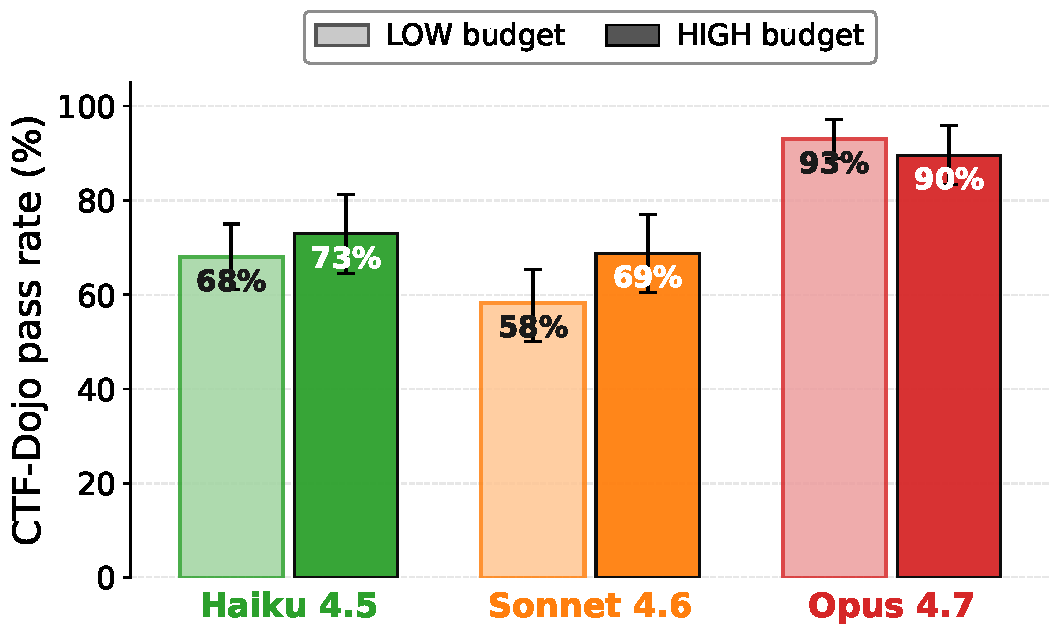
\includegraphics[width=\columnwidth]{figures/figure_c2_final.pdf}
\caption{\textbf{Evolver capability on CTF-Dojo.} Pass rate improves with stronger evolver models; higher budget helps Haiku and Sonnet but gives little additional gain once Opus already reaches high performance.}
\label{fig:app_c2_evolver_budget}
\end{figure}

\noindent\textbf{Cross-domain workspace dilution.}
Figure~\ref{fig:app_polybench_dilution} compares PolyBench CWR when using workspaces evolved on different domains. The PolyBench-specific workspace performs best, while the all-evolved workspace loses 57 points of CWR, showing that mixing heterogeneous experience can dilute domain-relevant harness structure.

\begin{figure}[t]
\centering
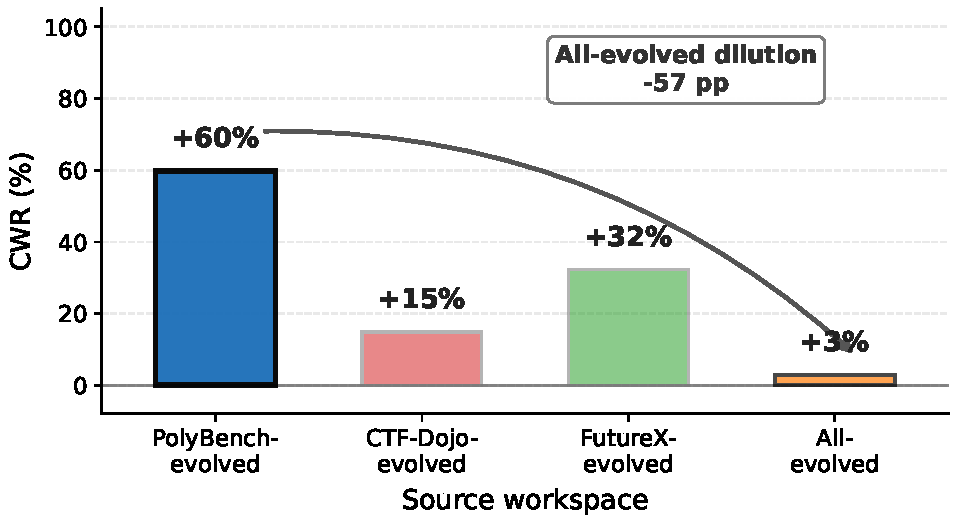
\includegraphics[width=\columnwidth]{figures/figure_c3_polybench_dilution.pdf}
\caption{\textbf{PolyBench workspace dilution.} A PolyBench-evolved workspace reaches the highest CWR, while combining all evolved workspaces sharply reduces CWR, supporting the need for specialized harness branches rather than a single dense harness.}
\label{fig:app_polybench_dilution}
\end{figure}

\FloatBarrier
\clearpage
\onecolumn
\section{Simplified Prompt Interfaces}
\label{app:prompts}

\newcommand{\PromptBlock}[2]{%
  \par\smallskip
  \begingroup
  \setlength{\fboxsep}{6pt}%
  \setlength{\fboxrule}{0.4pt}%
  \noindent\fcolorbox{black!35}{black!3}{%
    \begin{minipage}{0.94\linewidth}
    {\large\textbf{#1}}\par\vspace{0.25em}
    {\normalsize #2}
    \end{minipage}}%
  \par\smallskip
  \endgroup
}

The full prompts contain benchmark-specific paths and implementation details. We report simplified versions here to show the role structure and information flow used by Adaptive Auto-Harness.

\PromptBlock{Solve-time router}{
\textbf{Input:} the incoming task and branch summaries. \textbf{Instruction:} read each branch's intended scope, match the task to positive and negative routing signals, and select exactly one harness branch. Use the main branch when multiple branches match weakly or no branch has clear evidence. Return a branch name, confidence, and short reason.
}

\PromptBlock{Analyst}{
\textbf{Input:} recent trajectories, revealed feedback, branch statistics, and the persistent evolution workspace. \textbf{Instruction:} identify recurring failure patterns, separate transferable fixes from branch-specific fixes, and write a task board with priorities and targets. Audit stale or over-specialized artifacts before proposing new changes.
}

\PromptBlock{Researcher}{
\textbf{Input:} an analyst-assigned failure pattern or benchmark bottleneck. \textbf{Instruction:} search for candidate tools, APIs, data sources, or implementation strategies; test whether each candidate works under the benchmark constraints; and record concise findings that the builder can directly use.
}

\PromptBlock{Builder}{
\textbf{Input:} the task board, verified research records, current solver workspace, and architecture notes. \textbf{Instruction:} implement only the changes supported by verified research, update prompts, tools, memory, or infrastructure as needed, and preserve existing working code unless a targeted replacement is justified.
}

\PromptBlock{Verifier}{
\textbf{Input:} the builder's changes, target failure pattern, and benchmark constraints. \textbf{Instruction:} run focused tests before the changes go live, check that the implementation respects temporal filtering and sandbox rules, and return a pass/fail verdict with the concrete failure reason when retry is needed.
}

